% Conceptual figures only: synthetic 16x16 field, not an experimental result.
\begin{figure*}[t]
  \centering
  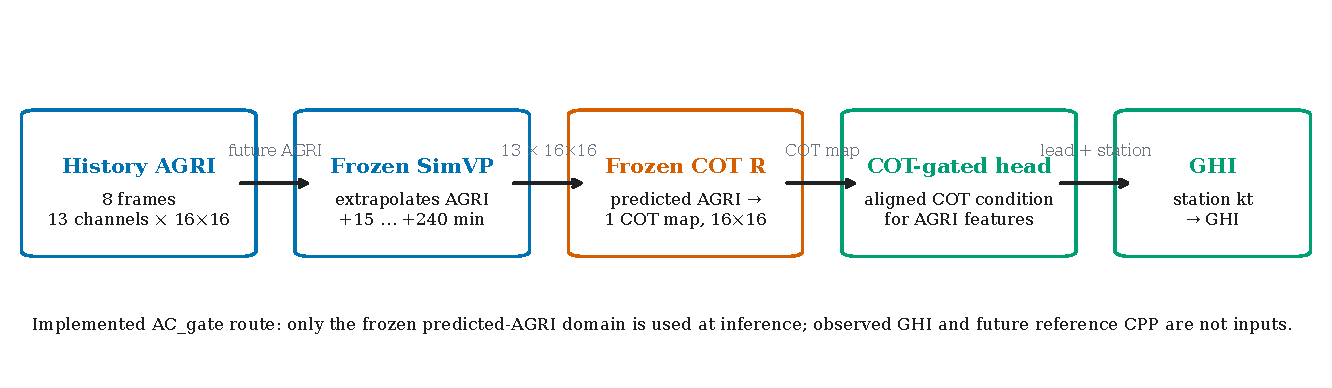
\includegraphics[width=\textwidth]{figures/cot_pipeline_20260918/fig_cot_pipeline_overview_20260918.pdf}
  \caption{Deployable route of the current AC\_gate candidate. Historical AGRI is extrapolated by frozen SimVP; the predicted AGRI is passed to the frozen COT retriever, whose aligned 16$\times$16 COT map conditions the station GHI head.}
  \label{fig:cot-pipeline-overview}
\end{figure*}

\begin{figure*}[t]
  \centering
  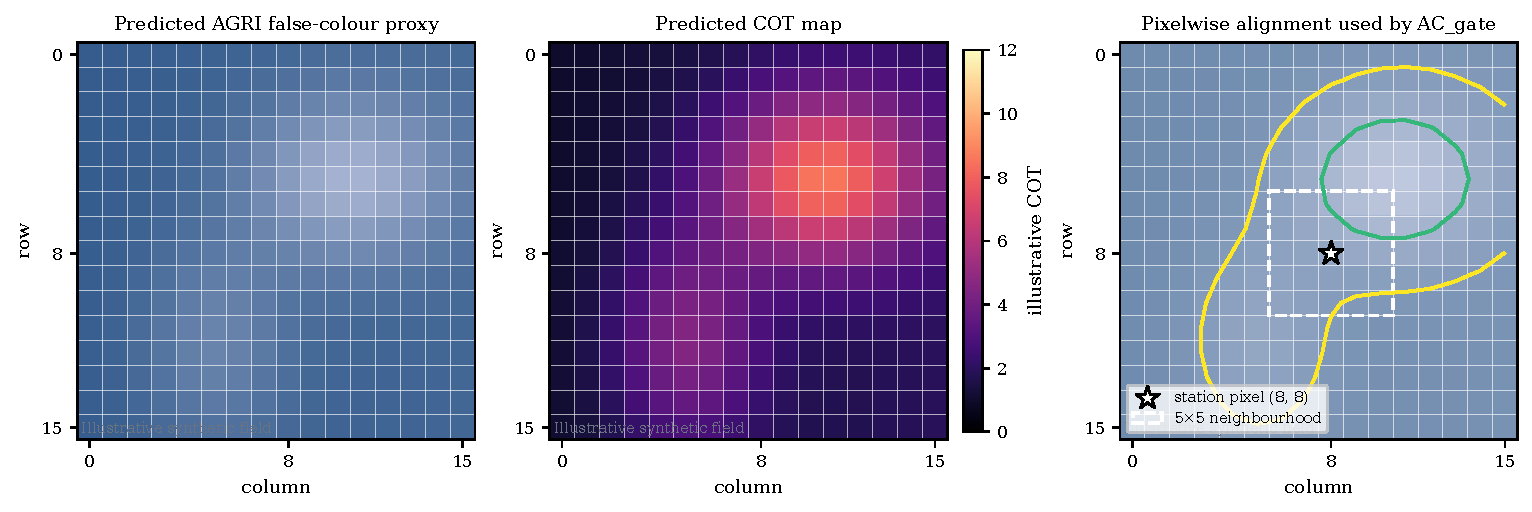
\includegraphics[width=\textwidth]{figures/cot_pipeline_20260918/fig_cot_patch_alignment_20260918.pdf}
  \caption{Conceptual 16$\times$16 alignment used by the AC\_gate candidate. The displayed field is synthetic and only explains the same-grid AGRI/COT representation, the station pixel, and its 5$\times$5 neighbourhood.}
  \label{fig:cot-patch-alignment}
\end{figure*}

\begin{figure*}[t]
  \centering
  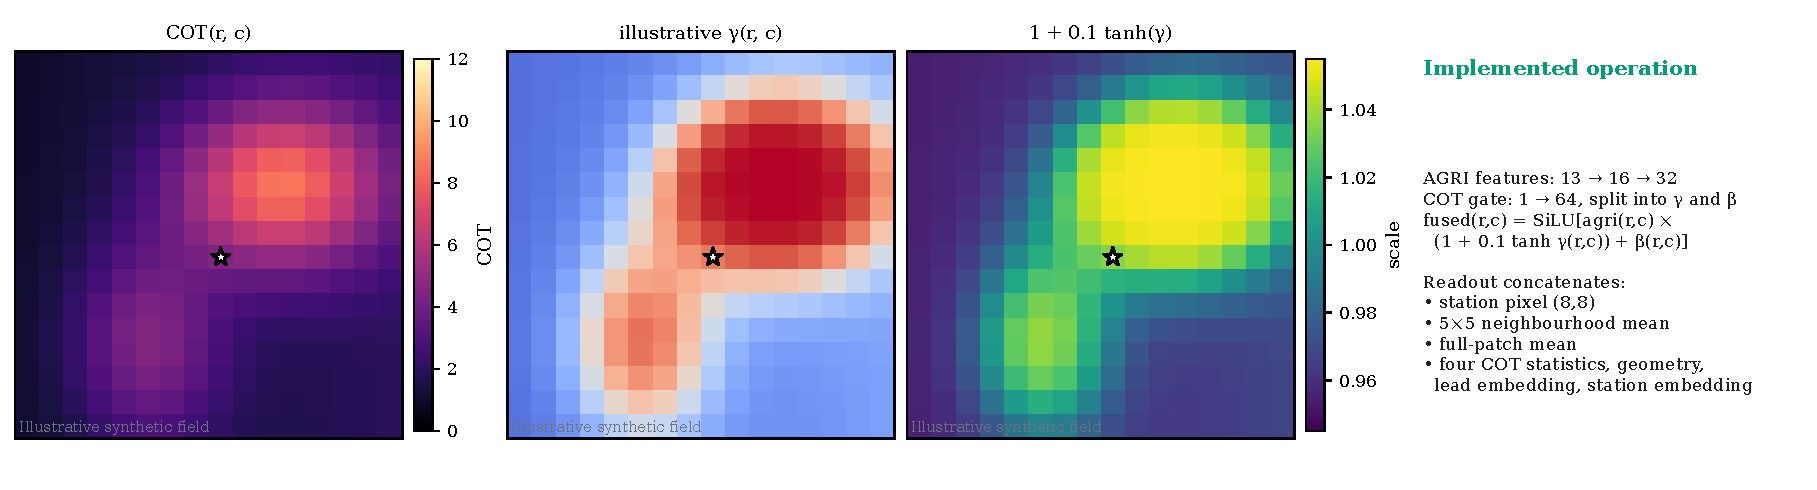
\includegraphics[width=\textwidth]{figures/cot_pipeline_20260918/fig_cot_pixel_gate_20260918.pdf}
  \caption{Conceptual pointwise COT conditioning and station-aware readout. The displayed $\gamma$ field is illustrative rather than a learned model output.}
  \label{fig:cot-pixel-gate}
\end{figure*}
